\chapter{Análisis y preprocesamiento}\label{chapter:methods}

Este capítulo está dedicada a detallar el análisis exploratorio sobre el conjunto de datos HeadQA y el preprocesamiento requerido. El capítulo está organizado en dos partes principales. La primera sección está dedicada a la planificación del proyecto presentando un esquema de pasos y tareas que fueron llevados a cabo en la realización de este trabajo, y que engloba desde el análisis del problema inicial hasta la presentación de los resultados. 

Las siguientes secciones están dedicadas al análisis descriptivo, transformación y modelización de los datos a utilizar con el objetivo de prepararlos para que sean una entrada válida a los modelos de aprendizaje que se presentan más adelante.

\section{Descripción CRISP-DM}

Esta sección está dedicada a la presentación de las diferentes fases del proyecto. Para la organización de este trabajo se sigue la metodología CRISP-DM (del inglés, \textit{Cross Industry Standard Process for Data Mining}), seguida con el objetivo de organizar el proceso de desarrollo. A continuación, se detalla a grandes rasgos el ciclo de vida del proyecto y las diferentes fases. 

El proyecto consta de las siguientes fases:

\begin{itemize}
  \item Comprensión del negocio
  \item Comprensión de los datos
  \item Preparación de los datos
  \item Modelado
  \item Evaluación
\end{itemize}

A continuación se describen brevemente las diferentes fases del proyecto, de igual manera en la Figura \ref{crisp} se muestran los pasos de manera gráfica y se detallan las actividades desarrolladas en cada caso.\\

\textbf{Comprensión del Negocio}: En esta fase inicial se define y entiende el problema en cuestión, planteado en la Introducción del trabajo. Asimismo, se trazan el objetivo general y los objetivos específicos para dar respuesta a la pregunta científica. Se realiza un estudio minucioso del estado del arte de los sistemas Q/A que permite no solo la comprensión del problema sino las principales formas de solución.

\textbf{Comprensión de los Datos}: La fase de entendimiento de datos comienza con la colección de datos inicial y continúa con las actividades que permiten familiarizarse con los datos, identificar los problemas de calidad y descubrir conocimiento preliminar sobre los datos a través de un análisis descriptivo.

\textbf{Preparación de los Datos}: La fase de preparación de datos cubre todas las actividades necesarias para construir el conjunto final a partir de los datos en bruto iniciales. Las tareas incluyen la transformación, la limpieza y la vectorización de datos para la modelación.

\textbf{Modelado}: En esta fase, se seleccionan y aplican las técnicas de modelado que sean pertinentes al problema en cuestión. Se diseñan e implementan las diferentes arquitecturas de red y algoritmos de aprendizaje automático.

\textbf{Evaluación}: Finalmente, en esta etapa del proyecto se evalúan los modelos anteriormente implementados y se comparan entre sí. Se analizan los resultados obtenidos cuantitativamente y también cualitativamente teniendo en cuenta su alineación con los objetivos inicialmente propuestos.

\begin{figure}[!tb]
  \begin{center}
    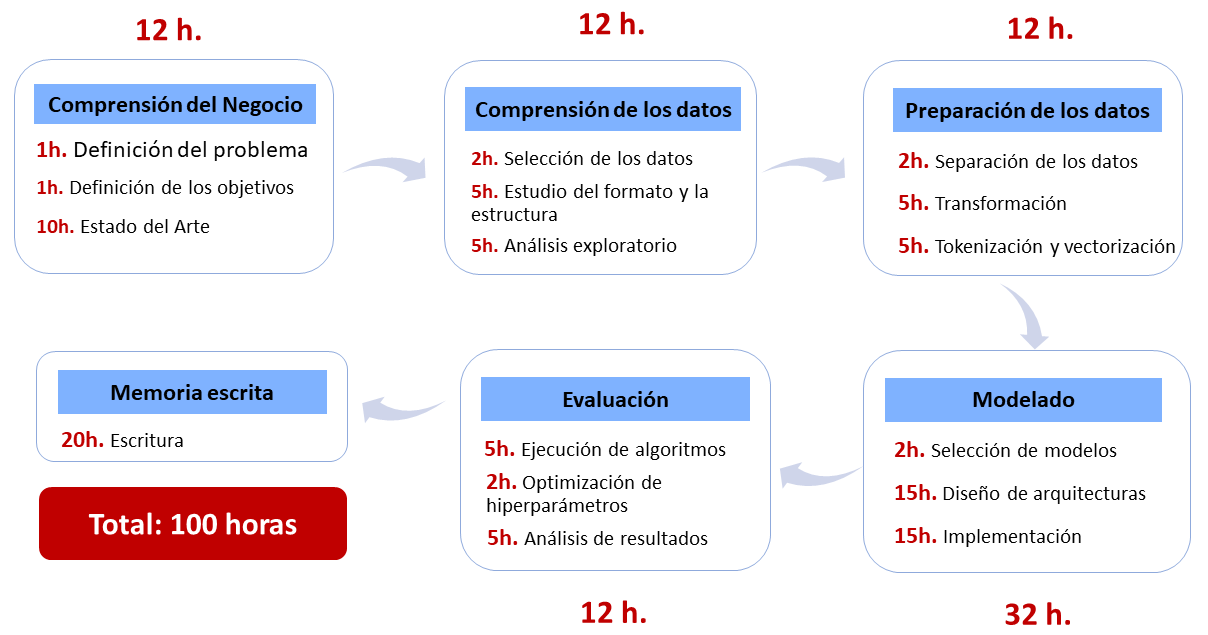
\includegraphics[angle=0, width=1\textwidth]{Graphics/crisp.png}
  \end{center}
    \caption{Etapas y tiempos de desarrollo del proyecto}\label{crisp}
\end{figure}

En la Figura \ref{crisp} se pueden visualizar cada una de las fases de desarrollo del proyecto, incluyendo las actividades específicas que se desarrollaron en cada etapa y la cantidad de horas dedicadas. A las fases anteriormente señaladas se añade la escritura de la memoria, haciendo un total de 100 horas.

\subsection{Descripción del conjunto de datos}

El conjunto de datos Head-QA presentado por \cite{2019-head-qa} y orientado al dominio biomédico, es un conjunto de preguntas y respuestas de múltiples opciones. El conjunto se crea a partir de los exámenes confeccionados por el Ministerio de Sanidad, Consumo y Bienestar Social de España \footnote{https://www.mscbs.gob.es} y realizados cada año para acceder a distintas especialidades dentro del sistema de salud. Más información sobre la confección del \textit{dataset} puede ser encontrada en \cite{2019-head-qa}.

Cada instancia del conjunto de datos está compuesta en esencia por una pregunta y las posibles respuestas, de las cuales solo una es correcta. Las preguntas y respuestas están organizadas en las categorías: Medicina, Enfermería, Biología, Química, Psicología, y Farmacología, correspondientes a los diferentes exámenes que se realizan. Aunque todas las propuestas publicadas hasta el momento se han construido sobre el paradigma no supervisado, el conjunto de datos está dividido en \textit{train}, \textit{development} y \textit{test}.

En la Figura \ref{sample} se muestra un ejemplo de pregunta/respuesta del \text{dataset}. 

\begin{figure}[!tb]
  \begin{center}
    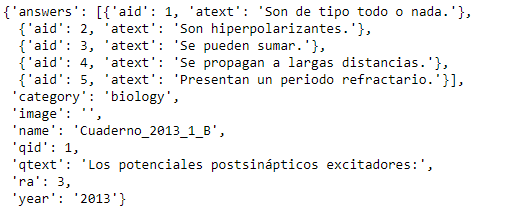
\includegraphics[angle=0, width=1\textwidth]{Graphics/sample.png}
  \end{center}
    \caption{Ejemplo de instancia del conjunto de datos}\label{sample}
\end{figure}

Cada instancia del conjunto está en formato JSON y contiene los siguientes atributos:

\begin{itemize}
  \item name: nombre del examen
  \item qid: identificador de la pregunta
  \item qtext: texto de la pregunta
  \item category: categoría del examen (Medicina, Enfermería, Biología, ...)
  \item year: año del examen
  \item answers: lista de posibles respuestas, conformada por su número y el texto
  \item ra: número de la respuesta correcta
  \item image: camino a la imagen si lo hay
\end{itemize}

Aunque en el idioma inglés se han realizado avances en la selección de respuestas y existen varios conjuntos de datos que permiten la evaluación de los modelos propuestos, incluso en ese idioma, los \textit{datasets} de dominios específicos y tan complejos como el actual son escasos. 

\section{Análisis descriptivo}

En esta sección se presenta un análisis exploratorio sobre el conjunto de dato sobre el cual se construirán los modelos. Aunque los algoritmos diseñados sobre estos datos hasta el momento han seguido el enfoque no supervisado y/o supervisado a distancia, los autores han presentado una partición con el fin de que pueda ser utilizado por algoritmos supervisados.

En total, Head-QA cuenta con 6.765 preguntas con sus respuestas posibles, organizadas en 6 categorías según la temática. La Tabla \ref{size} muestra la distribución de las instancias teniendo en cuenta las categorías y los subconjuntos de datos.

\begin{table}[!tb]
  \begin{center}
    \caption{Distribución de las preguntas en HeadQA}
    \begin{tabular}{l|c|c|c|c|c}
      \textbf{Categoría} & \textbf{Distribución total} & \textbf{Train} & \textbf{Dev} & \textbf{Test} \\
      \hline
      Biología & 1.132 & 452 & 226 & 454 \\
      Enfermería & 1.069 & 384 & 230 & 455 \\
      Farmacología & 1.139 & 457 & 225 & 457 \\
      Medicina & 1.149 & 455 & 231 & 463 \\
      Psicología & 1.134 & 453 & 226 & 455 \\
      Química & 1.142 & 456 & 228 & 458 \\ 
      \textbf{Total} & \textbf{6.765} & \textbf{2.657} & \textbf{1.366} & \textbf{2.742}\\
    \end{tabular}
  \end{center}
  \label{size}
\end{table}

Asimismo, la Figura \ref{train_dev_test} muestra la distribución de preguntas por categorías en los subconjuntos \textit{train}, \textit{dev} y \textit{test} de manera gráfica.

\begin{figure}[!b]
  \begin{center}
    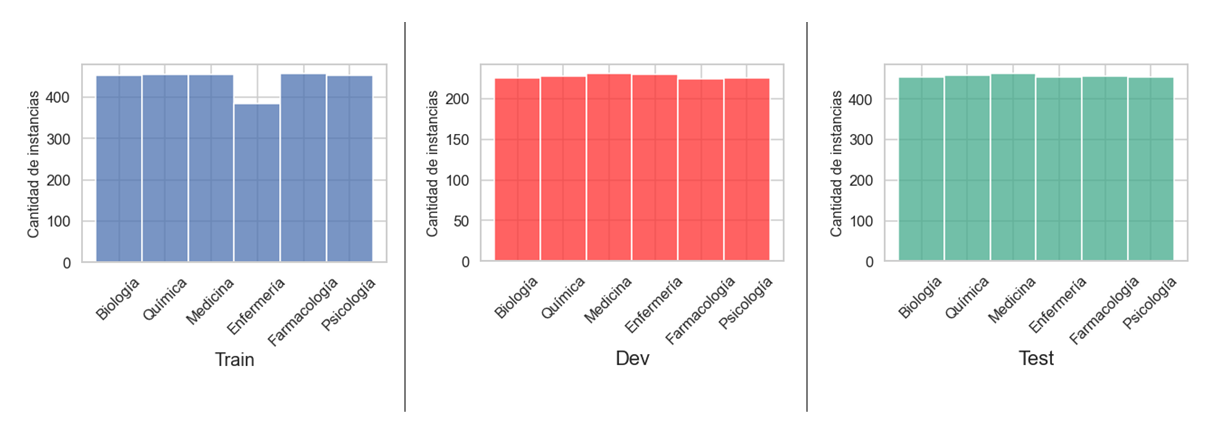
\includegraphics[angle=0, width=1\textwidth]{Graphics/train_dev_test.png}
  \end{center}
    \caption{Distribución de instancias por categoría}\label{train_dev_test}
\end{figure}

Se puede apreciar que las instancias están distribuidas de manera uniforme entre todas las categorías. Aunque el conjunto de datos está balanceado en cuanto a la cantidad de instancias por categoría, existen diferencias entre las muestras en las categorías como se muestra más adelante en cuanto a las palabras más comunes empleadas en los diferentes dominios del conocimiento.

\begin{figure}[!tb]
  \begin{center}
    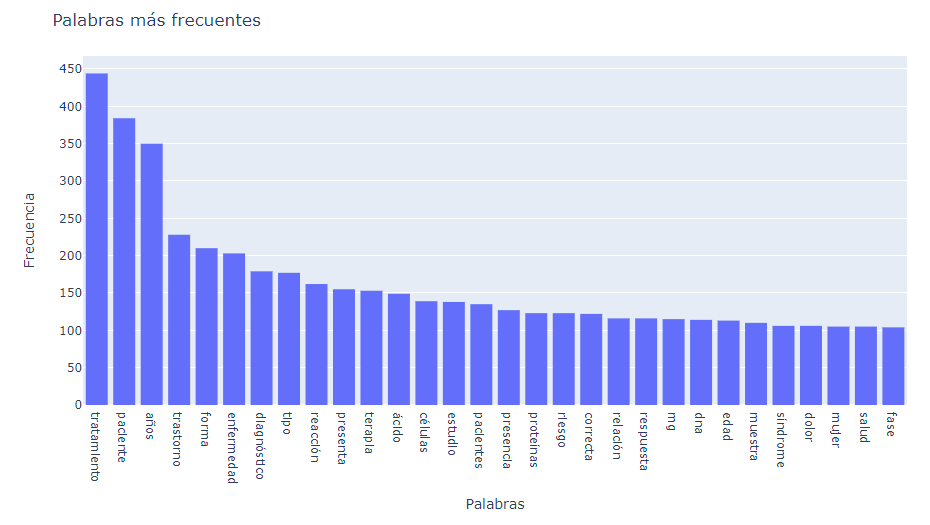
\includegraphics[angle=0, width=1\textwidth]{Graphics/words.png}
  \end{center}
    \caption{Palabras más frecuentes}\label{words}
\end{figure}

La Figura \ref{words} muestra la frecuencia de las palabras más comunes en el conjunto de entrenamiento. Mientras que que la Figura \ref{category} muestra la misma información mediante una nube de palabras por cada una de las categorías que definen el dominio de cada pregunta. 

La nube de palabras es un tipo de representación comúnmente utilizada cuando los datos son textuales y muestra las palabras que más se repiten en el dataset en mayor tamaño. De manera, que las palabras que destacan pueden ser interpretadas como las más importantes del dataset. Es importante destacar que para este análisis se eliminaron los \textit{stopwords} con el objetivo de centrarnos en las palabras propias del contexto.

\begin{figure}[!tb]
  \begin{center}
    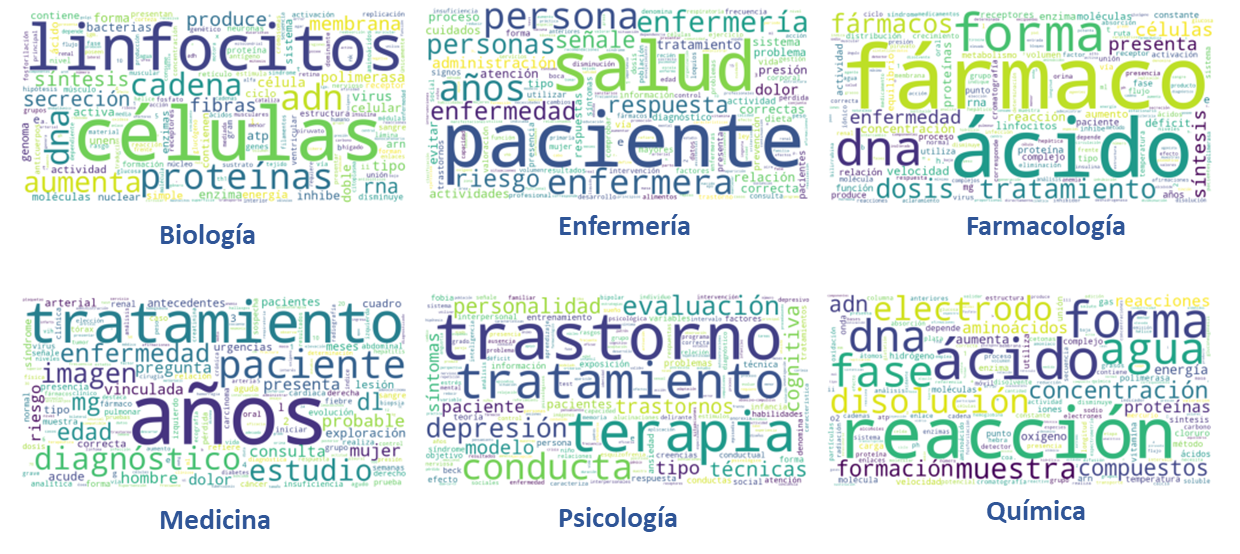
\includegraphics[angle=0, width=1\textwidth]{Graphics/word_category.png}
  \end{center}
    \caption{Nube de palabras por categoría}\label{category}
\end{figure}

Como se puede observar, las palabras más comunes difieren en gran medida de categoría a categoría. Esto sugiere que puede ser recomendable construir modelos independientes para cada uno de los dominios. Además, tras analizar la frecuencia de las palabras en el conjunto general se puede notar que existe una gran coincidencia entre las palabras más comunes en todo el conjunto de datos con las palabras de mayor mención en el subconjunto correspondiente a la temática Medicina, lo que sugiere que las preguntas de Medicina utilizan un vocabulario muy repetitivo o que estos términos son también empleados en las preguntas del resto de materias. 

La Tabla \ref{count} muestra la máxima y media cantidad de palabras que tienen las preguntas y las respuestas respectivamente.

\begin{table}[!tb]
  \begin{center}
    \caption{Tamaño de las preguntas y respuestas}
    \begin{tabular}{l|c|c|c|c|c}
      \textbf{Categoría} & \textbf{Max. pregunta} & \textbf{Avg. pregunta} & \textbf{Max. respuesta} & \textbf{Avg. respuesta} \\
      \hline
      Biología & 43 & 11 & 40 & 5 \\
      Enfermería & 187 & 29 & 94 & 9 \\
      Farmacología & 104 & 18 & 43 & 6 \\
      Medicina & 308 & 55 & 85 & 9 \\
      Psicología & 103 & 21 & 43 & 7 \\
      Química & 63 & 15 & 52 & 7 \\     
    \end{tabular}
  \end{center}
  \label{count}
\end{table}

Este análisis denota que las preguntas suelen tener una longitud media mayor que las respuestas. La longitud media varía en dependencia de la categoría, siendo los textos de Medicina los de mayor tamaño. Este hecho puede ser aprovechado en la construcción de los modelos independientes.

Tras un análisis exploratorio sobre el conjunto de datos es pertinente recurrir al procesamiento con el fin de convertir los datos textuales en entradas válidas y comprensibles para los modelos que se presentarán en el capítulo siguiente. 

\section{Preprocesamiento}

Como se plantea en el capítulo anterior, una instancia del corpus en esencia está conformada por la oración correspondiente a la pregunta, las correspondientes a las posibles respuestas y la respuesta correcta. Con el propósito de utilizar el corpus antes descrito como entrada a los modelos matemáticos que se presentan es necesario transformar cada una de las instancias en un vector numérico. En este caso, es necesario transformar las oraciones en una secuencia de \textit{tokens}.

En el idioma español, un \textit{token} constituye una cadena de caracteres consecutivos entre dos espacios, o entre un espacio y un signo de puntuación. Todos los signos constituyen \textit{tokens} excepto las comillas alrededor de una palabra, sin espacios intermedios, que simbolizan citas textuales. El conjunto de los \textit{tokens} presentes en el corpus constituye el vocabulario de palabras, donde a cada \textit{token} del vocabulario se le hace corresponder un número entero único. De esta manera, cada \textit{token} es representado por el índice de la palabra en el vocabulario de palabras. En este caso, el vocabulario de palabras está compuesto por todas las palabras que aparecen en el conjunto de datos, tanto en preguntas como en respuestas, junto a un conjunto de \textit{tokens} especiales.

Acorde con los modelos a desarrollar más adelante, se hace necesario emplear dos enfoques diferentes para vectorizar una instancia del conjunto de datos. El primero se ajusta a arquitecturas propias del aprendizaje supervisado, mientras que el segundo combina técnicas de recuperación de información en arquitecturas de aprendizaje supervisado. Cada uno de los enfoques requiere un preprocesamiento y representación de la información diferentes, los cuales se detallan a continuación.

\begin{figure}[!t]
  \begin{center}
    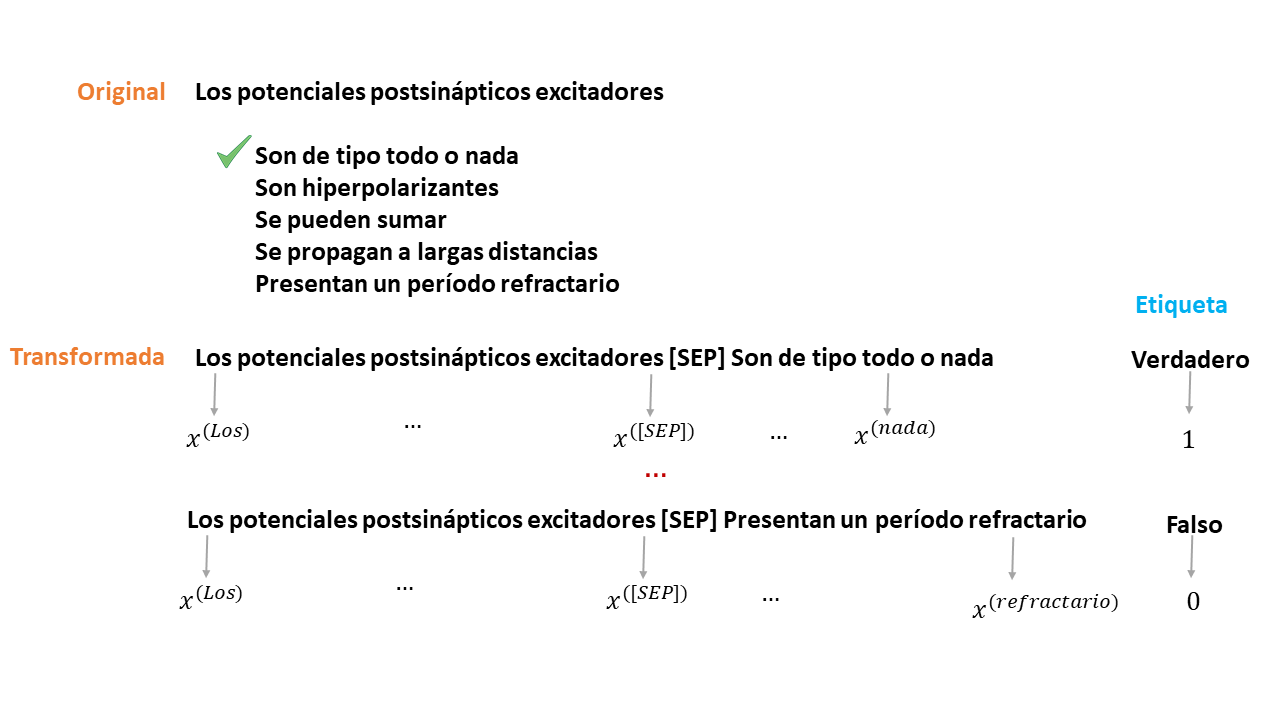
\includegraphics[angle=0, width=1\textwidth]{Graphics/vect_1.png}
  \end{center}
    \caption{Ejemplo de instancia vectorizada según el enfoque supervisado clásico}\label{vect_1}
\end{figure}

\subsection{Representación supervisada clásica}

Este enfoque consiste en que los modelos reciban un único vector numérico, por lo tanto el objetivo es representar en un mismo vector la pregunta y cada respuesta.

Siguiendo los métodos \textit{Pointwise} donde el problema de selección de respuestas se transforma en un problema de clasificación binario, a partir de una instancia del conjunto de datos original se construyen varios ejemplos vectorizados (ver Figura \ref{vect_1}). 

Cada instancia original se transforma en tantos vectores como respuestas posibles haya (pueden ser 4 o 5, dependiendo del examen). De manera que cada nuevo ejemplo vectorizado está formado por el texto de la pregunta y el texto de la respuesta separados por un carácter especial, introducido en el vocabulario de palabras con ese objetivo. Se le asigna 1 como etiqueta si el par $(pregunta, respuesta)$ es verdadero, en caso contrario, se le asigna la etiqueta negativa.

En la Figura \ref{vect_1} se muestra como una instancia del conjunto original es transformada en vectores numéricos, teniendo en cuenta la pregunta y si la respuesta es correcta o no.

Con el objetivo de transformar una oración en una secuencia de \textit{tokens} es necesario utilizar un \textit{tokenizer}. Un \textit{tokenizer} no es más que un algoritmo cuyo objetivo es separar texto en bruto en una secuencia de \text{tokens}. En este caso, se utiliza el tokenizador de la librería Spacy\footnote{https://spacy.io/}, específicamente el modelo \texttt{es\_core\_news\_sm}. Este modelo es el más pequeño disponible en español, se selecciona el más pequeño porque la tarea de tokenizar no es muy complicada en términos lingüísticos por lo que la autora considera que no es necesario utilizar otro modelo más grande y complejo solo para realizar esta tarea.

\begin{figure}[!tb]
  \begin{center}
    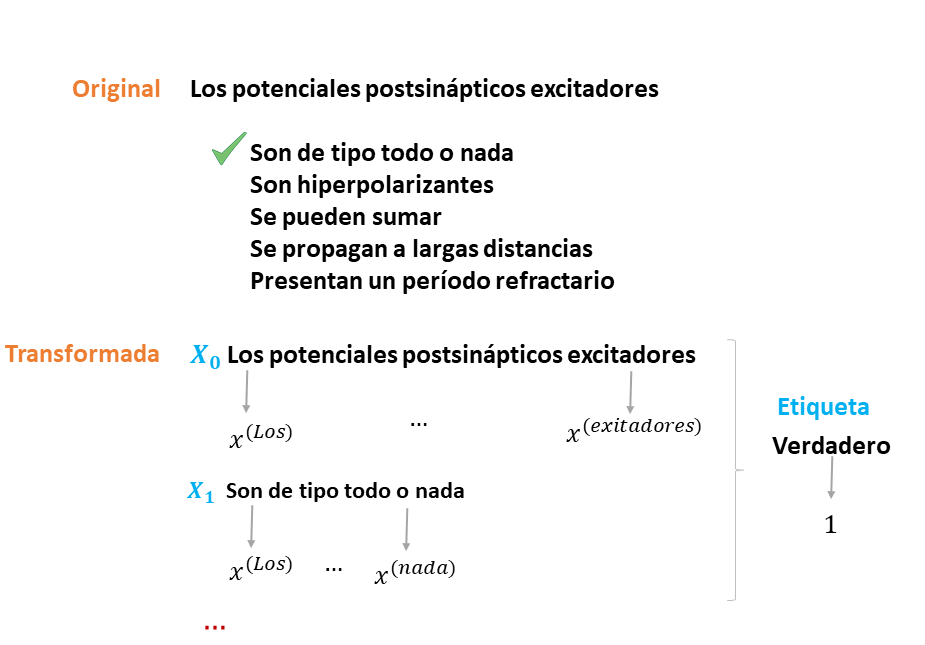
\includegraphics[angle=0, width=1\textwidth]{Graphics/vect_2.png}
  \end{center}
    \caption{Ejemplo de instancia vectorizada según el enfoque RI}\label{vect_2}
\end{figure}

\subsection{Representación supervisada RI}

El otro enfoque constituye una combinación entre el modelo vectorial clásico en el área de recuperación de información y un modelo de aprendizaje supervisado genérico.  En este caso, los modelos de este perfil en lugar de un único vector numérico que represente ambos textos, la pregunta y la respuesta, están preparados para recibir como entrada una representación vectorial de la pregunta y otra de la respuesta.

La transformación es muy similar a la vista en la sección anterior, con la diferencia de que al admitir dos entradas no es necesario concatenar ambas representaciones y por tanto, tampoco es necesario el \textit{token} especial que actúa como separador.

En la Figura \ref{vect_2} se muestra un ejemplo de cómo es transformada una instancia del conjunto original, en varias instancias vectorizadas. 

Al igual que en la situación anterior es necesario transformar las oraciones en bruto en una secuencia de \textit{tokens} y se utiliza el mismo \textit{tokenizer}.
Una vez transformado el texto en bruto en representaciones numéricas, los datos están preparados para ser tratados por los modelos matemáticos.   


Después del análisis, preprocesamiento y transformación del conjunto de datos original, los datos están listos para ser utilizados como entrada a los modelos. En el próximo capítulo se presentan varios modelos de aprendizaje supervisado, específicamente bajo el paradigma de aprendizaje profundo, los cuales constituyen propuestas de solución para resolver el problema de selección de respuestas en el idioma español sobre la base del corpus HeadQA detallado en el presente capítulo.


\chapter{Modelos propuestos}\label{chapter:models}

En el presente capítulo se propone interpretar el problema de selección de respuestas como un problema de clasificación binaria, según el enfoque \textit{Pointwise}, explicado en el Capítulo 1. Se ha seleccionado este enfoque por ser el más sencillo de los tres, y se propone para trabajos futuros incursionar en los demás métodos mencionados. En esta metodología cada par $<pregunta, respuesta>$ se convierte en una instancia y se clasifica en positiva o negativa dependiendo si la respuesta es correcta. Habiendo obtenido el corpus, el objetivo desde este punto es concebir modelos matemáticos-computacionales de aprendizaje profundo principalmente. En este capítulo se presentan diferentes propuestas de modelos para la selección automática de respuestas. 

La decisión de implementar modelos de aprendizaje profundo, existiendo modelos supervisados más sencillos y explicables, se basa en que tras un estudio de los modelos del estado del arte, se puede concluir que la mayor parte con diferencia emplea este enfoque. La razón se debe a que estos conjuntos de datos son más complejos semánticamente por lo que requieren un mayor entendimiento del lenguaje humano y por lo tanto, modelos mucho más complejos. 

De hecho, el aprendizaje supervisado puede no ser un enfoque adecuado para este conjunto de datos, puesto que como se afirma en \cite{2020-multi-step} incluso un modelo tan poderoso como BERT puede funcionar de manera insatisfactoria en el conjunto de datos HeadQA. La principal razón es que la pregunta inicial no contiene suficientes pistas recuperables para encontrar la respuesta correcta que contiene la respuesta y además, aunque exista una similitud entre los exámenes anteriores, puede no ser suficiente para generar patrones por un modelo supervisado.


\section{\textit{LSTM} Básico}\label{lstm_t}

La primera propuesta se puede considerar un modelo de aprendizaje profundo relativamente sencillo cuyo objetivo principal es verificar las ventajas que proporcionan las redes recurrentes en la resolución del problema de selección de respuestas.

La primera propuesta consiste en una red neuronal recurrente de tipo \textit{LSTM}, la cual recibe como entrada una oración vectorizada. La arquitectura se divide en tres capas: representación de los \textit{tokens}, representación de la oración y predicción de la etiqueta (respuesta correcta). En la Figura \ref{lstm} se presenta la arquitectura de la red correspondiente al modelo matemático que se expone a continuación. El modelo matemático solo se incluirá en este primer caso, puesto que su sencillez lo permite y a la vez, permite familiarizarnos con las arquitecturas recurrentes. 

\begin{figure}[!tb]
  \begin{center}    
    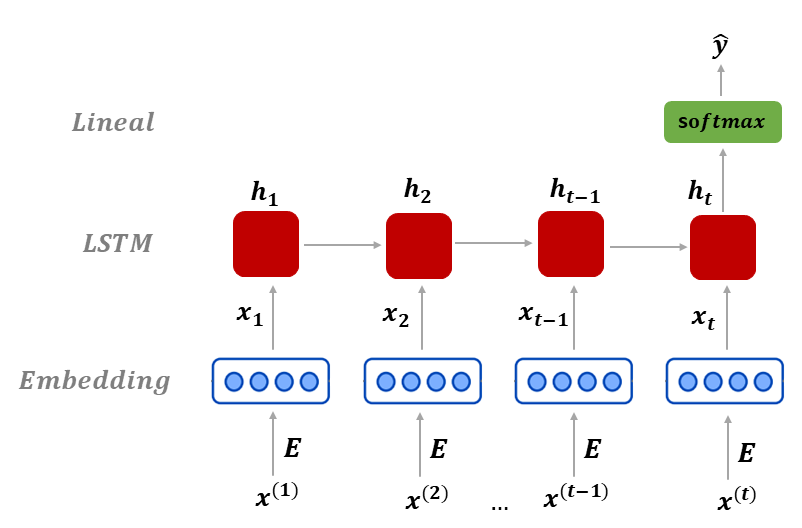
\includegraphics[angle=0, width=0.75\textwidth]{Graphics/lstm2.png} 
  \end{center}
    \caption{Arquitectura del modelo LSTM básico}\label{lstm}
\end{figure}

Sea $S = [x^{(1)}, x^{(2)}, ..., x^{(T)}]$ la representación vectorial de una oración $S$, donde $x^{(t)}$ representa el t-ésimo \textit{token} con $(t = 1, 2, ..., T)$ y $T$, la cantidad de \textit{tokens} de la oración. El modelo puede ser definido formalmente como:

\begin{align}
  x_{t} &= Ex^{(t)} \label{lstm:emb} \\
  \nonumber \\
  i_{t} &= \sigma{(W^{(i)} x_{t} + U^{(i)}h_{t-1})} \label{lstm:ig} \\
  f_{t} &= \sigma{(W^{(f)} x_{t} + U^{(f)}h_{t-1})} \label{lstm:fg} \\
  o_{t} &= \sigma{(W^{(o)} x_{t} + U^{(o)}h_{t-1})} \label{lstm:og} \\
  \tilde{c_{t}} &= \tanh(W^{(c)} x_{t} + U^{(c)}h_{t-1}) \label{lstm:new_memory_generation} \\
  c_{t} &= f_{t}c_{t-1} + i_{t}\tilde{c_{t}} \label{lstm:cell_state} \\
  h_{t} &= o_{t}\tanh{c_{t}} \label{lstm:hidden_state} \\
  \nonumber \\
  \hat{y} &= sigmoid(Uh_{T} + b) \label{lstm:pred}
\end{align}

En una primera etapa (Ecuación \ref{lstm:emb}), el modelo obtiene una representación más rica semánticamente de cada uno de los \textit{tokens} que conforman una oración. Esto se logra a través de una capa de \textit{embeddings} $E$ que transforma cada \textit{token} $x^{(t)}$ en un vector $x_{t}$ $\in$ ${\mathbb{R}} ^{d}$, donde $d$ es la dimensión de los \textit{embeddings} que constituye un hiperparámetro del modelo.

En la segunda etapa (Ecuaciones \ref{lstm:ig} - \ref{lstm:hidden_state}), el modelo procesa la secuencia de \textit{tokens} para obtener una representación final de la oración. Esto se logra con la inclusión de una capa \textit{LSTM}, la cual analiza de manera secuencial cada una de las salidas $x_{t}$ de la capa de \textit{embeddings}. El centro de una red \textit{LSTM} es el funcionamiento de sus celdas, una red \textit{LSTM} tiene tantas celdas como \textit{tokens} tiene una oración. Las Ecuaciones \ref{lstm:ig} - \ref{lstm:hidden_state} describen el comportamiento de una celda de la red \textit{LSTM}. En la tabla \ref{tab:cell_state} se describe la notación empleada.

\begin{table}[!tb]
  \center \caption{Descripción de símbolos utilizados en una red \textit{LSTM}}
    \begin{center}
      \begin{tabular}{|c|l|}
        \hline
        \textbf{Símbolo} & \textbf{Significado}\\
        \hline
        $x_{t}$ & entrada a la celda \textit{LSTM} en el paso $t$ \\
        $h_{t-1}$ & salida de la celda \textit{LSTM} en el paso $t-1$ \\
        $i_{t}$ & valor de la \textit{input gate} en el paso $t$\\
        $f_{t}$	& valor de la \textit{forget gate} en el paso $t$ \\
        $o_{t}$	& valor de la \textit{output gate} en el paso $t$\\
        $\sigma$ & función sigmoidal\\
        $W^{(\alpha)}$ & pesos de $x_{t}$ en $\alpha_t$ ($\alpha = {i, f, o}$) \\
        $U^{(\alpha)}$ & pesos de $h_{t-1}$ en $\alpha_t$ ($\alpha = {i, f, o}$) \\
        $\tilde{c_{t}}$ & candidato a \textit{cell state} en el paso $t$\\
        $c_{t}$ & \textit{cell state} en el paso $t$ \\
        $h_{t}$ & salida final de la celda \textit{LSTM} en el paso $t$ \\
        $h_{T}$ & salida final de la celda \textit{LSTM} en el último paso $T$ \\
        \hline
        \end{tabular}
    \end{center}
    \label{tab:cell_state}
\end{table}

Una celda \textit{LSTM} está compuesta por tres componentes fundamentales:
\begin{itemize}
  \item La \textit{input gate}, en español "válvula de entrada", expresada en la Ecuación \ref{lstm:ig}, tiene la función de determinar qué información debe estar presente en el estado de la celda (en inglés, \textit{cell state}) representado por $c_{t}$, teniendo en cuenta la salida final de la celda anterior $h_{t-1}$.
  \item La \textit{forget gate}, en español "válvula del olvido", representada en la Ecuación \ref{lstm:fg}, tiene la función de determinar qué información es irrelevante en el estado de la celda $c_{t}$; funciona de manera análoga a la \textit{input gate}.
  \item La \textit{output gate}, en español "válvula de salida", representada en la Ecuación \ref{lstm:og}, tiene la función de determinar el nivel de activación del estado $c_{t}$ para la salida final.
\end{itemize}

En todos estos casos, se utiliza como función de activación la función sigmoide $\sigma$ con el propósito de que los valores sean positivos y se encuentren entre 0 y 1.

La Ecuación \ref{lstm:new_memory_generation}, conocida como \textit{new memory generation} o \textit{candidate cell}, calcula un estado recurrente temporal $\tilde{c_{t}}$ teniendo en cuenta la entrada $x_{t}$ y el estado anterior $h_{t-1}$. En este caso, para superar el problema de \textit{vanishing gradient}\footnote{https://towardsdatascience.com/the-vanishing-gradient-problem-69bf08b15484} se necesita una función de activación cuya segunda derivada pueda mantenerse durante un largo rango antes de llegar a cero, razón por la cual se utiliza la tangente.

En la Ecuación \ref{lstm:cell_state} se calcula el estado de la celda actual $c_{t}$ teniendo en cuenta qué debe olvidar del estado previo a través de la expresión $f_{t}*c_{t-1}$ y qué debe considerar del estado actual temporal representado en la expresión $i_{t}*\tilde{c_{t}}$. En la Ecuación \ref{lstm:hidden_state} se toma el estado de la celda $c_{t}$ y la \textit{output gate} $o_{t}$ para determinar qué información queda contenida en el estado último de la celda $h_{t}$.

Es importante destacar que los parámetros $E$, $W^{(i)}$, $W^{(f)}$, $W^{(o)}$, $W^{(c)}$, $U^{(i)}$, $U^{(f)}$, $U^{(o)}$, $U^{(c)}$ y $U$ son aprendidos durante la etapa de entrenamiento en el proceso de \textit{backpropagation}.

Las operaciones presentadas en las ecuaciones \ref{lstm:ig} - \ref{lstm:hidden_state} son ejecutadas $T$ veces, por cada uno de los \textit{tokens} que conforman una oración. Tras el análisis del último \textit{token} $T$, el estado final $h_{T}$ constituye una representación de la oración $S$. Finalmente, una capa lineal (Ecuación \ref{lstm:pred}) utiliza la representación de la oración obtenida $h_{T}$ para predecir la relación $\hat{y}$ existente en la oración. Esta salida se convierte en una robabilidad empleando la función \textit{sigmoid}. Esta operación, a diferencia de las ecuaciones anteriores, solo se aplica una vez al estado final $h_{T}$ de la capa \textit{LSTM}.

La sencillez arquitectónica del modelo permite que se pueda utilizar como base para la comparación con otros modelos más complejos que serán abordados a continuación.

\section{\textit{BiLSTM+Att}}\label{bilstm_t}

El segundo modelo propuesto tiene una arquitectura más compleja que el anterior consistiendo, esencialmente, en una red \textit{BiLSTM} integrada con un mecanismo de atención.

En este caso, se adiciona el uso de un modelo del lenguaje (en inglés, \textit{language model})  (\cite{mikolov-2016-fastext}) pre-entrenado en un conjunto de documentos en idioma español con el propósito de ganar riqueza semántica en la representación de la oración. Utilizar un modelo pre-entrenado ofrece la posibilidad de aprovechar el conocimiento del lenguaje contenido en la representación de las palabras (a través de los \textit{embeddings} pre-entrenados en una tarea auxiliar) en nuestra tarea específica que, en este caso, es la selección de respuestas. El modelo del lenguaje empleado es el presentado por \cite{mikolov-2016-fastext}, entrenado sobre un conjunto de artículos médicos de la biblioteca electrónica \textit{Scielo}\footnote{https://scielo.isciii.es/scielo.php} tomados de \cite{2019-medical-fastext}.

Las redes recurrentes unidireccionales en general, en el análisis de una palabra, tienen en cuenta solo las palabras anteriores (o posteriores), sin embargo sería útil que al hallar la representación de una palabra se tuviera en cuenta tanto las palabras que aparecen antes como las que aparecen después en una oración. Por esta razón se decide utilizar una capa \textit{BiLSTM}, esto posibilita que en cada estado de una secuencia, la red tenga una visión completa y consecutiva de todos los estados anteriores y posteriores. Se propone la inclusión de una capa de atención pues podría ayudar al modelo a darle más peso a ciertas palabras en la oración que pueden ser determinantes en la predicción.

En la Figura \ref{bilstm} se expone la arquitectura de la red correspondiente al modelo que se presenta en esta sección. 

\begin{figure}[!tb]
  \begin{center}
    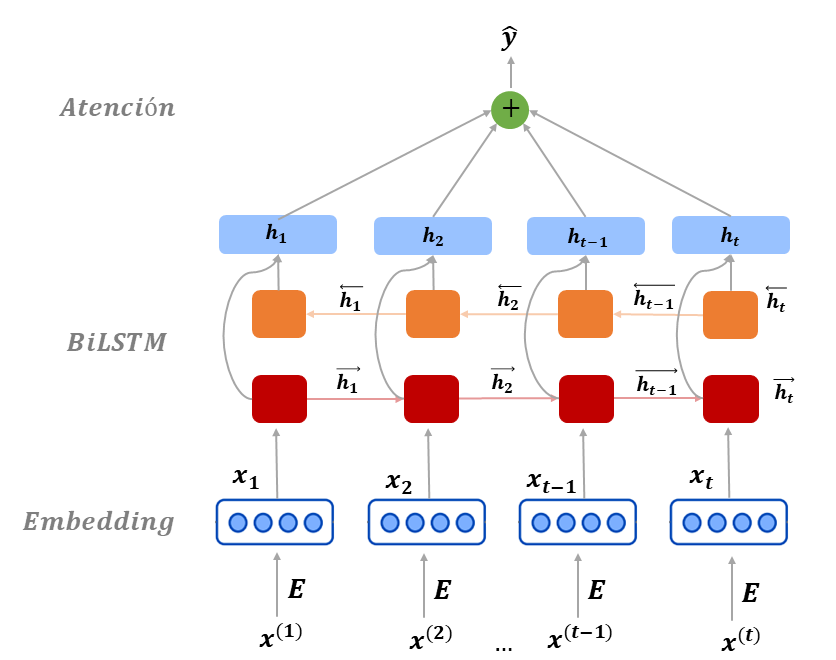
\includegraphics[angle=0, width=0.75\textwidth]{Graphics/bilstm.png}
  \end{center}
    \caption{Arquitectura del modelo \textit{BiLSTM+Att}}\label{bilstm}
\end{figure}

El modelo contiene una primera capa de \textit{embeddings} pre-entrenada que transforma el \textit{word index} en una representación más rica semánticamente representada como un vector de dimensión establecida. La diferencia en esta primera capa con respecto al modelo anterior se  encuentra en que en el modelo \textit{LSTM} los pesos de la capa de \textit{embeddings} $E$ se aprenden durante la etapa de entrenamiento, mientras que, en este caso, los pesos que se utilizan pertenecen a \textit {embeddings} pre-entrenados tomados de \cite{2019-medical-fastext} que ya contienen un conocimiento del idioma español y del dominio médico específicamente, adquirido previamente.

Una segunda capa está conformada por una red \textit{Bi-LSTM}, la cual permite tener en cuenta para el cómputo de un estado no solo las palabras anteriores sino también las siguientes. Posteriormente, se incluye la capa de atención. El objetivo de incluir un mecanismo de atención es que el modelo dé mayor peso a aquellas palabras que tienen una mayor influencia en la predicción final, de manera que su resultado es un vector de pesos, llamado vector de pesos de atención, que es combinado linealmente con la representación de las oraciones que se tenía en la capa anterior dando como resultado un nuevo vector, conocido como vector contexto, que constituye la representación final de la oración. Finalmente, una capa lineal utiliza la representación de la oración obtenida para predecir si la respuesta es correcta o no.

\section{QA-LSTM}

Este modelo hace uso de las redes bidireccionales y a su vez emplea un enfoque clásico del área de recuperación de información, está inspirado en el introducido por \cite{2015-tan-qalstm}, aunque con algunas diferencias. En la Figura \ref{lstm_qa} se presenta la arquitectura del modelo. Es importante destacar que mientras las arquitecturas presentadas anteriormente combinaban la pregunta y la respuesta en una misma entrada, los modelos que se presentan a partir de este momento utilizan una representación separada para pregunta y respuesta. Por esta razón, en la figura se presentan dos veces la misma arquitectura, cuyo objetivo es codificar el texto perteneciente a la pregunta y a la respuesta por separado, aunque en la práctica se utiliza la misma red para ambos textos.

Ambas arquitecturas, notables en la base de la red por capas, comparten la misma arquitectura. Se ha visualizado de esta forma para lograr una mejor comprensión por parte del lector.

\begin{figure}[!tb]
  \begin{center}
    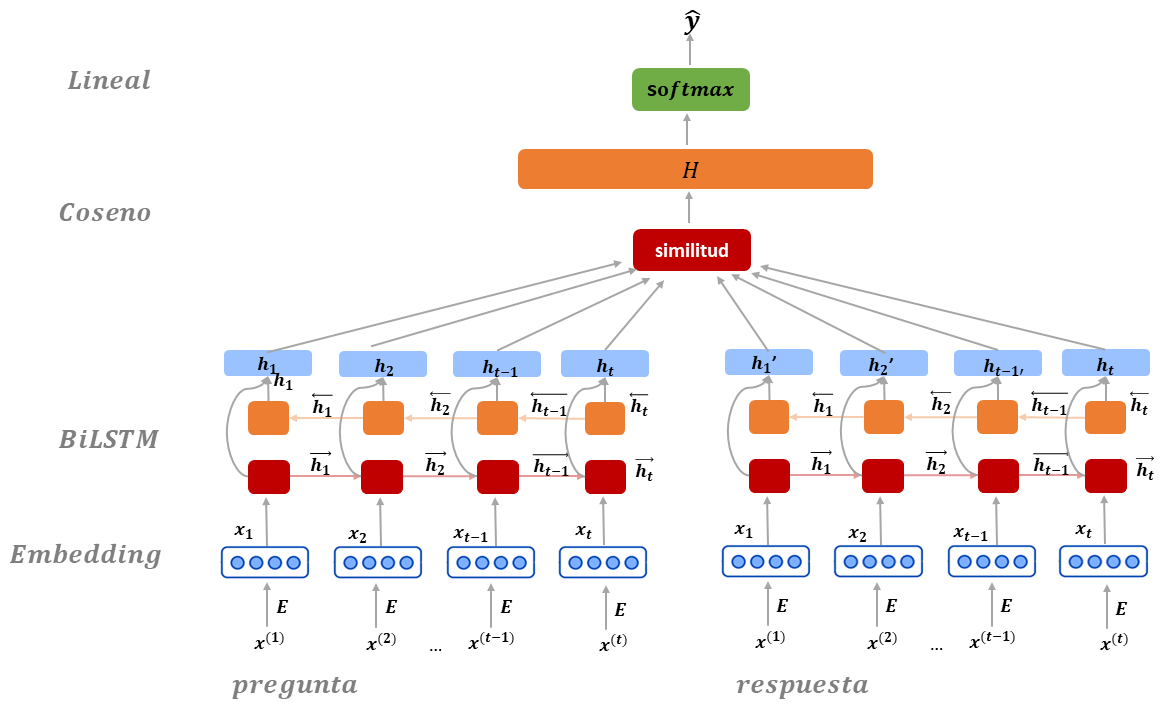
\includegraphics[angle=0, width=1\textwidth]{Graphics/lstm_qa.png}
  \end{center}
    \caption{Arquitectura del modelo QA-LSTM}\label{lstm_qa}
\end{figure}

El modelo contiene una primera capa de \textit{embeddings} pre-entrenada que transforma el \textit{word index} en una representación más rica semánticamente representada como un vector de una dimensión fija para cada palabra. Al igual que en el modelo \textit{BiLSTM+Attn} se utilizan embeddings pre-entrenados, se toman como base para la capa de \textit{Embeddings} los vectores palabras orientados al dominio biomédico citados anteriormente y publicados por \cite{2019-medical-fastext}.

Estos embeddings se utilizan como entrada a una capa LSTM bidireccional. La red BiLSTM genera representaciones distribuidas tanto para la pregunta como para la respuesta de forma independiente, y luego utilizan la similitud del coseno para medir su distancia. 

Como se muestra en la figura y se explicó anteriormente en la introducción de las redes recurrentes de tipo LSTM, al aplicar este tipo de redes es posible obtener una representación de cada palabra a través de los estados intermedios y que brindan el atributo de recurrencia. De esta manera, en cada palabra tenemos un vector resultado de analizar las palabras anteriores y que se puede interpretar como una representación de dicha palabra en el contexto de sus antecesoras. Como estamos en presencia de una red recurrente bidireccional, en cada momento se cuenta con dos vectores, uno que constituye la representación de esa palabra a partir de sus anteriores y otros, a partir de sus posteriores. 

En el modelo que se expone se utilizan todos los estados intermedios de la red para representar cada oración. Esto implica que tenemos dos vectores para la pregunta y dos para la respuesta, la representación final de cada una de las oraciones se obtiene concatenando los pares con que se contaba. A partir de estas representaciones de calcula la similitud del coseno resultando igualmente en un vector. Por último, este vector es conectado con una capa de regresión linear que utiliza \textit{sigmoid} como función de activación, de manera que la salida en un número entre 0 y 1. Esta salida puede ser interpretada como el nivel de relevancia de la respuesta con la pregunta, y es necesario establecer un punto de corte para determinar si la instancia es positiva o negativa.

\section{QA-LSTM/CNN}

En esta sección se expone el modelo QA-LSTM/CNN, el cual es muy similar al anterior y su arquitectura fue también introducida por \cite{2015-tan-qalstm}. En la Figura \ref{lstm_cnn_qa} se muestra de manera gráfica la arquitectura de este modelo. Como se puede apreciar es muy parecida a la arquitectura presentada anteriormente, la única diferencia es la inclusión de una capa convolucional tras las redes bidireccionales.

\begin{figure}[!tb]
  \begin{center}
    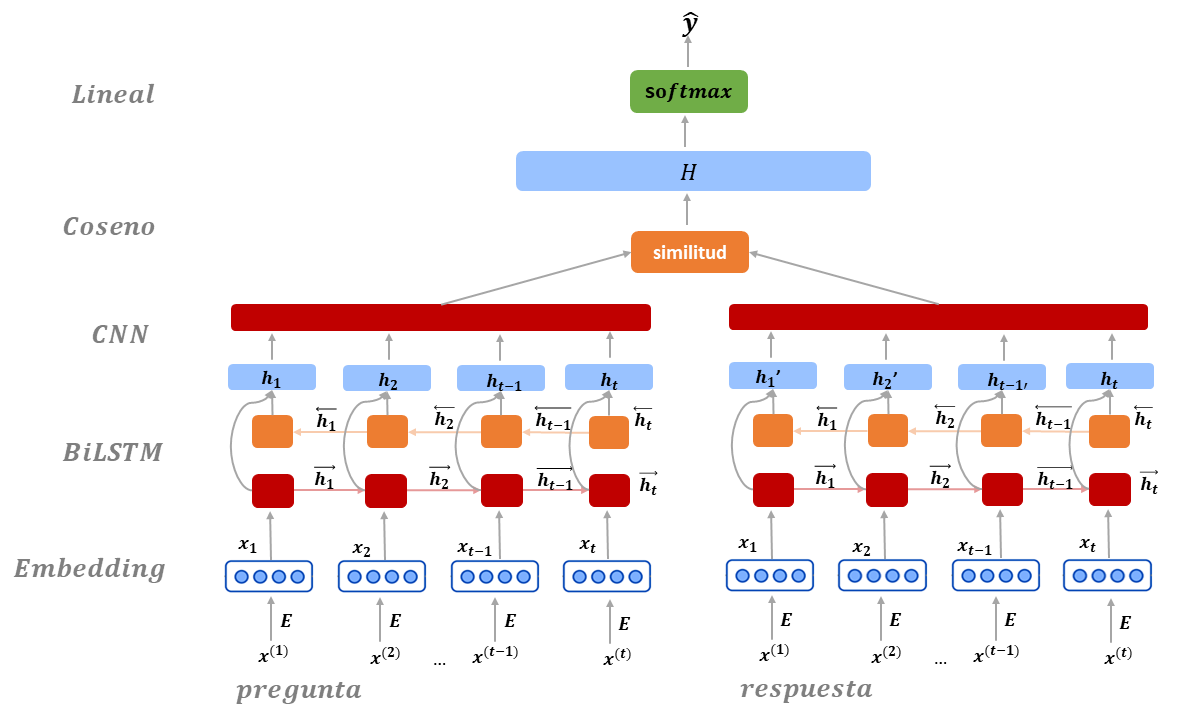
\includegraphics[angle=0, width=1\textwidth]{Graphics/lstm_cnn_qa.png}
  \end{center}
    \caption{Arquitectura del modelo QA-LSTM/CNN }\label{lstm_cnn_qa}
\end{figure}

En la sección anterior, las representaciones de preguntas y respuestas se generan solo por simple operaciones, en este caso, la concatenación. Este nuevo modelo recurre a una estructura de CNN construida sobre los resultados de BiLSTM, con el fin de ofrecer una representación más compacta de las preguntas y las respuestas. A diferencia de la red neuronal tradicional, donde cada salida es interactiva con cada entrada, la estructura convolucional solo impone interacciones locales entre las entradas dentro de un tamaño de filtro $m$. Eesto quiere decir que la representación resultante tiene en cuenta la interacción de las palabras más cercanas, tanto a la derecha como a la izquierda.

Se decide incorporar esta arquitectura porque los autores de \cite{2015-tan-qalstm} señalan que alcanzan resultados superiores que con la arquitectura anterior. Sin embargo, aunque esto es una razón para incluirla en la experimentación no asegura el éxito dadas las diferencia de los contextos.  

\section{QA-BERT: \textit{Transfer Learning}}\label{bert_t}

\cite{2018-devlin-bert} plantea que el uso de BERT en el enfoque \textit{fine tuning} obtiene nuevos resultados en el estado del arte en varias tareas de procesamiento del lenguaje natural, entre ellas, el reconocimiento de entidades nombradas y los sistemas pregunta/respuesta.

La diferencia con otros modelos de representación del lenguaje, en cuanto a arquitectura, es que BERT está basado en un \textit{Transformer} bidireccional. En el artículo de \cite{2018-devlin-bert} no se detalla la arquitectura del modelo \textit{Transformer}. Otra diferencia es que modifica la tarea tradicional de \textit{language modeling} sobre la que se entrena introduciendo nuevas tareas. La primera tarea introducida recibe el nombre de \textit{masked language model} y consiste en ocultar palabras aleatorias en un texto y predecir, teniendo en cuenta el contexto, el \textit{token} que corresponde a la posición oculta, mientras que la segunda tarea consiste en, dada una oración en un texto, predecir la oración siguiente.

Los autores de BERT señalan como principal contribución la demostración de la efectividad del pre-entrenamiento bidireccional en la representación del lenguaje sobre las arquitecturas unidireccionales utilizadas hasta ese momento y, además, plantean que con el uso de esta nueva representación se puede reducir la complejidad de la arquitectura del modelo y aún así, obtener mejores resultados.

El modelo que se presenta en esta sección comparte la esencia del modelo QA-LSTM, pero en lugar de utilizar un red de tipo BiLSTM en las capas bases, utiliza un modelo BERT pre-entrenado. Los autores de BERT en su trabajo \cite{2018-devlin-bert} afirman que el uso de BERT trae consigo una riqueza semántica mayor que los embeddings tradicionales. Aunque no fue probado formalmente que BERT tiene conocimiento del lenguaje humano, los resultados sugieren que este modelo posee una capacidad de entendimiento del lenguaje mayor que modelos vistos con anterioridad.

Bajo esta suposición, se considera que la representación que se puede lograr con BERT tanto de las preguntas como de las oraciones, puede tener más información del idioma español en general, dada la cantidad de información con que fue entrenado este sistema. El modelo BERT base que se utiliza fue entrenado sobre un corpus en idioma español presentado por \cite{2020-spanish-bert}. En la Figura \ref{bert_qa} se muestra gráficamente la arquitectura del modelo que se presenta.

\begin{figure}[!tb]
  \begin{center}
    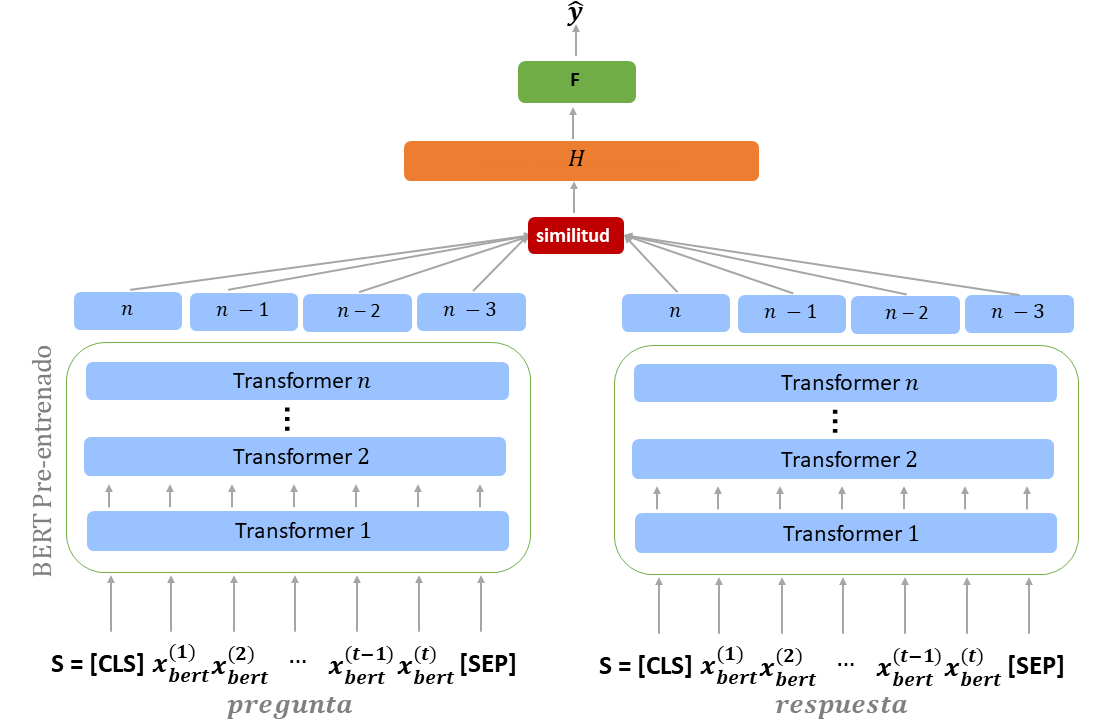
\includegraphics[angle=0, width=1\textwidth]{Graphics/bert_qa.png}
  \end{center}
    \caption{Arquitectura del modelo BERT-QA}\label{bert_qa}
\end{figure}

BERT es básicamente una pila de codificadores de arquitectura \textit{Transformer}, como se muestra en la base de la imagen. Una arquitectura \textit{Transformer} es una red de codificador-decodificador basadas en diferentes mecanismos de atención. BERT BASE, la versión más ligera, tiene 12 capas en la pila del codificador, mientras que BERT LARGE tiene 24 capas en la pila del codificador. \cite{2020-spanish-bert}, modelo que se utiliza en esta propuesta, utiliza la arquitectura BERT BASE.

En esta arquitectura se propone utilizar la salida de la última capa de BERT como representación tanto de la pregunta como la respuesta y sobre estas representaciones aplicar las mismas operaciones que en el caso de LSTM-QA. Luego de obtener las representaciones contextuales se aplica una medida de similitud, obteniendo un vector que es utilizado para dar la predicción final de la instancia, a través de una capa \textit{fully connected} con función de activación sigmoidal, cuya salida puede interpretarse nuevamente como la relevancia de la posible respuesta a la pregunta.


\subsection{Especificidad del preprocesamiento}

Con el objetivo de transformar una oración en un vector computacionalmente interpretable, anteriormente se propuso un preprocesamiento que fue aplicado a los modelos de aprendizaje presentados. Sin embargo, en el caso de BERT, las oraciones no pueden ser traducidas a vectores numéricos de la misma forma que se hizo en las propuestas anteriores, sino que BERT requiere un formato diferente. Con el fin de obtener los resultados esperados, el corpus original siempre debe ser modificado en función de las pautas planteadas por los autores en \cite{2018-devlin-bert}. Asimismo, el \textit{tokenizer} empleado no puede ser el mismo que el utilizado para los modelos anteriores, puesto que BERT tiene un vocabulario de palabras diferentes.

BERT define los siguientes \textit{tokens} especiales para la representación de una oración. Dichos \textit{tokens} reciben una interpretación diferente en la etapa de entrenamiento.
\begin{itemize}
  \item \textbf{[CLS]}: Indica el inicio de una oración
  \item \textbf{[SEP]}: Indica el fin de una oración
  \item \textbf{[MASK]}: Se utiliza para denotar \textit{tokens} que deben ser ignorados por el modelo
\end{itemize}

BERT no acepta secuencias de tamaño variable por lo que se recurre a la estrategia de \textit{padding}, en la que se establece un tamaño máximo. Las oraciones que tienen una cantidad menor de \textit{tokens} son completadas con el \textit{token} especial \textbf{[MASK]}, para indicar que esas posiciones deben ser ignoradas.

\section{BERT No Supervisado}

Las propuestas no supervisadas publicadas hasta el momento se apoyan en un gran conjunto de documentos textuales de las temáticas relacionadas. Las propuestas presentadas en \cite{2019-head-qa} y \cite{2020-multi-step}, las únicas a saber de la autora sobre este conjunto de datos, utilizan como fuente de información externa artículos de Wikipedia, artículos de la revista Scielo, entre otras. 

El gran volumen de datos que contienen estas bibliotecas hacen que el procesamiento sea muy costoso, tanto de recursos computacionales como de tiempo. Esta propuesta busca aprovechar los recursos y el tipo de procesamiento dedicados anteriormente proponiendo el uso de un modelo pre-entrenado. 

Se propone hallar una representación a partir de BERT, esta representación tiene incluida de alguna manera conocimiento sobre los documentos con que fue entrenado BERT. Una limitante es que dado el coste de entrenar desde cero un modelo como BERT no existen modelos entrenados en idioma español especializados en el dominio biomédico por lo que se utiliza el presentado por \cite{2020-spanish-bert}, que ha sido entrenado sobre un gran corpus de documentos en idioma español.

En la Figura \ref{bert_sim} se presenta la arquitectura del modelo en cuestión.

\begin{figure}[!tb]
  \begin{center}
    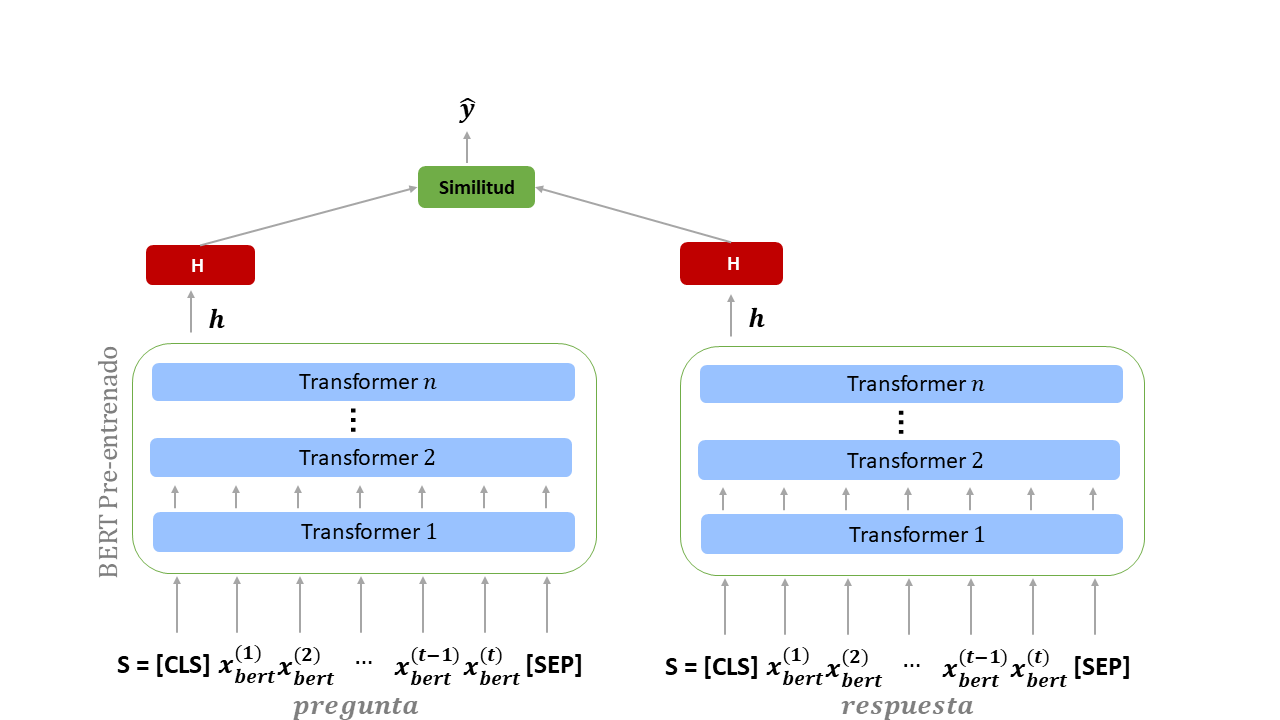
\includegraphics[angle=0, width=1\textwidth]{Graphics/bert_sim.png}
  \end{center}
    \caption{Arquitectura del modelo BERT-Sim}\label{bert_sim}
\end{figure}

La idea es utilizar BERT como codificador de las oraciones de entrada, tanto la pregunta como la respuesta, y posteriormente, aplicar un modelo vectorial clásico. Como se mencionó anteriormente BERT es básicamente una pila de codificadores de arquitectura \textit{Transformer}, como se muestra en la base de la imagen, cuya versión más ligera y la utilizada en este caso (publicada en \cite{2020-spanish-bert}), tiene 12 capas en la pila del codificador. 

El modelo que se propone codifica la pregunta y la respuesta por separado utilizando la salida de las últimas cuatro capas de BERT. Los vectores salida se concatenan de manera que se obtiene un vector de gran tamaño para cada oración. A partir de estos vectores se aplica el coseno del ángulo como medida de similitud, cuyo resultado es la salida del modelo y puede ser interpretado como el nivel de correspondencia entre la pregunta y la respuesta.

El objetivo de este modelo tan sencillo es comprobar si un modelo tan poderoso como BERT puede a través de la representación contextual de las palabras que obtiene y un modelo vectorial clásico ser aplicado eficazmente a la selección de respuestas.

\section{Implementación}\label{section:implementation}

En esta sección, se abordan los elementos esenciales para la programación y ejecución de los modelos propuestos y se describen de manera breve las herramientas utilizadas en el proceso de implementación.

En toda la solución se utilizó Python\footnote{http://www.python.org} como lenguaje de programación. Fue seleccionado porque debido a que el código es libre, existe una gran cantidad de bibliotecas implementadas por la comunidad de desarrolladores para dar respuesta a problemas diversos. De igual manera, Python constituye uno de los lenguajes más populares en el procesamiento del lenguaje natural. Contiene bibliotecas como Spacy\footnote{https://spacy.io/} y NLTK\footnote{https://www.nltk.org/} que cuentan con un gran número de funcionalidades implementadas. La completitud de Spacy y la facilidad de uso fueron determinantes en la selección como biblioteca para el procesamiento textual, empleada en la fase de preprocesamiento de las oraciones. 

Asimismo, Python contiene varias alternativas en cuanto a bibliotecas de aprendizaje profundo y ofrece opciones para la visualización y comparación de resultados. Keras\footnote{https://keras.io/}, TensorFlow\footnote{https://www.tensorflow.org/} y PyTorch\footnote{https://pytorch.org/} se encuentran entre los tres marcos principales preferidos por los científicos de datos y los principiantes en el campo del aprendizaje profundo. En este caso, se utiliza PyTorch para implementar los modelos de aprendizaje pues es una herramienta de más bajo nivel que posibilita el trabajo con tensores, facilitando la manipulación interna de las arquitecturas neuronales, a diferencia de Keras y TensorFlow, que ofrecen APIs más generales.

En el capítulo \ref{chapter:models} se presentó el proceso de concepción, modelación y diseño de los modelos a aplicar al problema de selección de respuestas como un problema de clasificación binario. Asimismo, se abordaron los detalles del proceso de implementación de los modelos expuestos. El próximo capítulo está dedicado a evaluar y comparar los modelos implementados en términos de métricas estándares para la evaluación de tareas de clasificación.





